
\documentclass[template=tabling,81pt,headonall]{azmoon}
\usepackage{xepersian}
\usepackage{amsfonts}
\usepackage{graphicx}
\usepackage{svg}
\svgpath{ {./images/} }
\graphicspath{ {./images/} }
\settextfont{Yas}
\setdigitfont{A Iranian Sans}
\usepackage{fontawesome5}

\printanswers
    \teacher{محمد صالح علی اکبری}
    \teachertitle{دبیر}
    \city{رحمت آباد}
    \schooltitle{متوسطه دوره اول}
    \school{مقداد}
    \grade{هشتم}
    \branch{}
    \topic{ریاضی}
    \examdate{۱۳/۰۳/۱۴۰۳}
    \answertime{۸۰ دقیقه}
    \begin{document}
	\begin{questions}
		\nointerlineskip%
		\vskip-\baselineskip
		\question[1.5]{%
حاصل تقسیم‌های زیر را تا ۲ رقم اعشار محاسبه کنید.
    \begin{LTR}
        \begin{parts}[3]\part{$\dfrac{25}{2} = $}
\part{$\dfrac{14}{28} = $}
\part{$\dfrac{18}{6} = $}
\end{parts}
\end{LTR}
        ‌
\\
    }\question[2]{%
مقدار $x$ و $y$ را با توجه به خطوط و زوایای زیر بدست آورید. \\ 
\includegraphics[scale = 0.5]{دو خط موازی} \\ 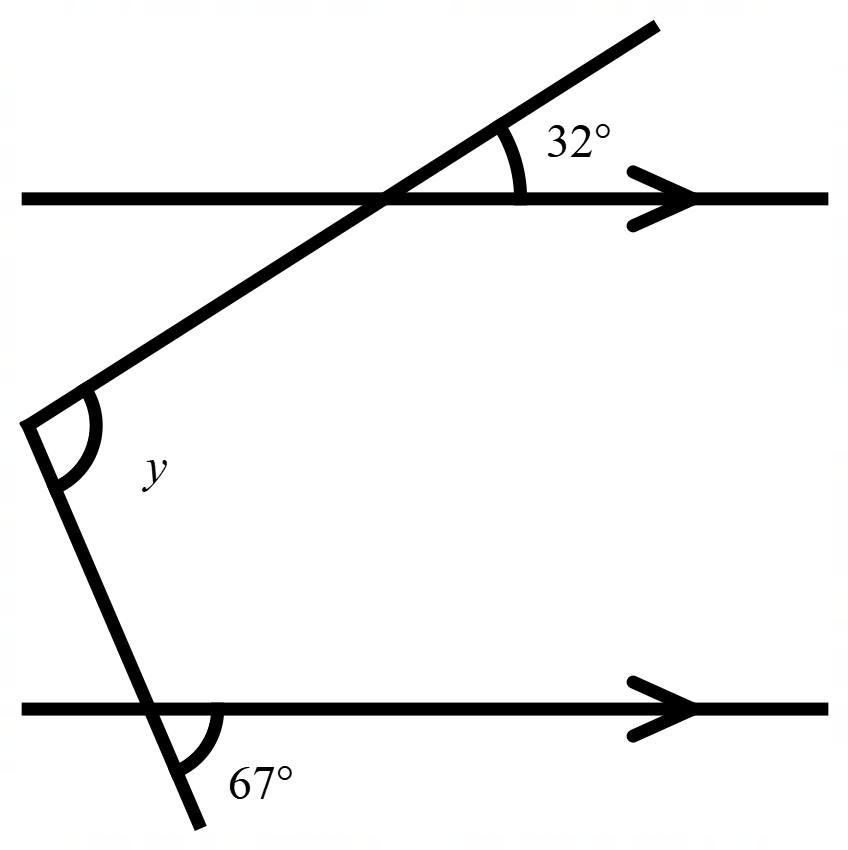
\includegraphics[scale = 0.5]{زاویه بین دو خط موازی}}\question[3]{%
حاصل جمع و تفریق‌های زیر را محاسبه کنید.
    \begin{LTR}
        \begin{parts}[1]\part{$\dfrac{3}{5}+\dfrac{7}{5} = $}
‌\\\part{$\dfrac{1}{5}-\dfrac{4}{5} = $}
‌\\\part{$\dfrac{2}{5}-\dfrac{2}{3} = $}
‌\\\part{$\dfrac{2}{7}+\dfrac{4}{6} = $}
\end{parts}
\end{LTR}
        ‌
\\
    }\question[1]{%
حاصل عبارت‌های زیر را محاسبه کنید.
    \begin{LTR}
        \begin{parts}[2]\part{$\sqrt{16} =$}
\part{$\sqrt{36} =$}
\end{parts}
\end{LTR}
        
    }\question[1]{%
حاصل عبارت‌های زیر را محاسبه کنید.
    \begin{LTR}
        \begin{parts}[2]\part{$3^3 =$}
\part{$2^4 =$}
\end{parts}
\end{LTR}
        
    }\question[3]{%
معادله‌های زیر را محاسبه کنید.
    \begin{LTR}
        \begin{parts}[2]\part{$4x + 3 = 2x + 5$}
\part{$2x + 3 = 3x + 1$}
‌\\‌\\\part{$22x + 5 = 13x - 4$}
\part{$12x + 15 = 3x - 14$}
\end{parts}
\end{LTR}
        ‌
\\‌
\\
    }\question[4]{%
معادله‌های زیر را محاسبه کنید.
    \begin{LTR}
        \begin{parts}[2]\part{$-\dfrac{3}{8}x+5=\dfrac{1}{6} $}
\part{$\dfrac{5}{12}x - \dfrac{7}{18} = 2$}
‌\\‌\\‌\\‌\\\part{$\dfrac{1}{2}-\dfrac{2x-1}{4} = \dfrac{3}{4}$}
\part{$4x + \dfrac{2}{7} = \dfrac{3}{2}x$}
\end{parts}
\end{LTR}
        ‌
\\‌
\\‌
\\‌
\\
    }\question[1]{%
کوچک ترین مضرب مشترک جفت اعداد زیر را محاسبه کنید.
    \begin{LTR}
        \begin{parts}[2]\part{$[12 , 8] = $}
\part{$[6 , 4] = $}
\end{parts}
\end{LTR}
        
    }\question[1]{%
بزرگ ترین مقسوم علیه مشترک جفت اعداد زیر را محاسبه کنید.
    \begin{LTR}
        \begin{parts}[2]\part{$(12 , 8) = $}
\part{$(16 , 4) = $}
\end{parts}
\end{LTR}
        
    }\question[1]{%
یک 7 ضعلی مجموع زوایای داخلی اش چقدر است؟‌
\\‌
\\}\question[1.5]{%
اندازه زاویه داخلی یک ۵ ضلعی منتظم چقدر است؟‌
\\‌
\\‌
\\}\end{questions}
    \end{document}
    